% don't remove the folling lines, and edit the defintion of \main if needed
\documentclass[../report.tex]{subfiles}
\providecommand{\main}{..}
\IfEq{\jobname}{\currfilebase}{\AtEndDocument{\biblio}}{}
% until here

\begin{document}
\section{Extended Higgs sectors and high-energy flavour dynamics}
\label{sec:BSM-ExtendedScalars}

This section presents the physics reach of future collider facilities in the areas of extended Higgs sectors, neutral naturalness, and high-energy flavour dynamics. Substantial improvements with respect to \HLLHC are possible for all included physics topics, and both direct and indirect searches typically provide complementary information. In several cases the combined interpretation of measurements in hadron and lepton collisions, at different stages of energy, enhance the physics potential even further.

\subsection{Extended Higgs sectors}
The scalar sector of the SM consists of one isospin doublet of scalar fields $H$ which contains the minimal set of required degrees of freedom: longitudinal polarisations of the $W$ and $Z$ bosons and the Higgs particle. However, many new-physics scenarios predict extended Higgs sectors, with one particle closely resembling the SM Higgs boson, and additional scalars.

A simple possibility is the extension of the SM scalar potential by a singlet massive scalar field $S$ with interactions $V= \lambda_{S}S^{4}/4+\lambda_{HS} |H|^{2}S^{2}$. 
This scenario is of particular interest, not just for its minimality, but also because  it can change the nature of the EW phase transition (see Sect.~\ref{chap:ew}). In the SM, the phase transition is a smooth crossover, whereas a strong first-order phase transition could open up new exciting possibilities, such as observable gravitational waves in future facilities or a framework for a mechanism generating the cosmic baryon asymmetry.

From the point of view of collider searches, there are two distinct singlet scenarios, depending on whether or not the singlet mixes with the Higgs. In the case where a heavy singlet mixes with the SM Higgs boson, direct limits on the mixing parameter $\sin \gamma$ for high-energy lepton~\cite{Buttazzo:2018qqp} and hadron colliders~\cite{Sirunyan:2018qlb, CidVidal:2018eel} are compared in Fig.~\ref{fig:singlets} (left). The overall scaling of the Higgs boson couplings~\cite{deBlas:2019rxi} provides an indirect probe even at colliders with $\sqrt{s}$ below the mass of the heavy singlet. At \HLLHC, \HELHC and CLIC direct and indirect searches provide complementary information, whereas the direct reach at \FCChh exceeds the sensitivity from Higgs-coupling measurements for masses up to 12\,TeV. Precision EW observables are not competitive with Higgs measurements and the corresponding reach is not shown in the figure.

\begin{figure}[ht]
\centering
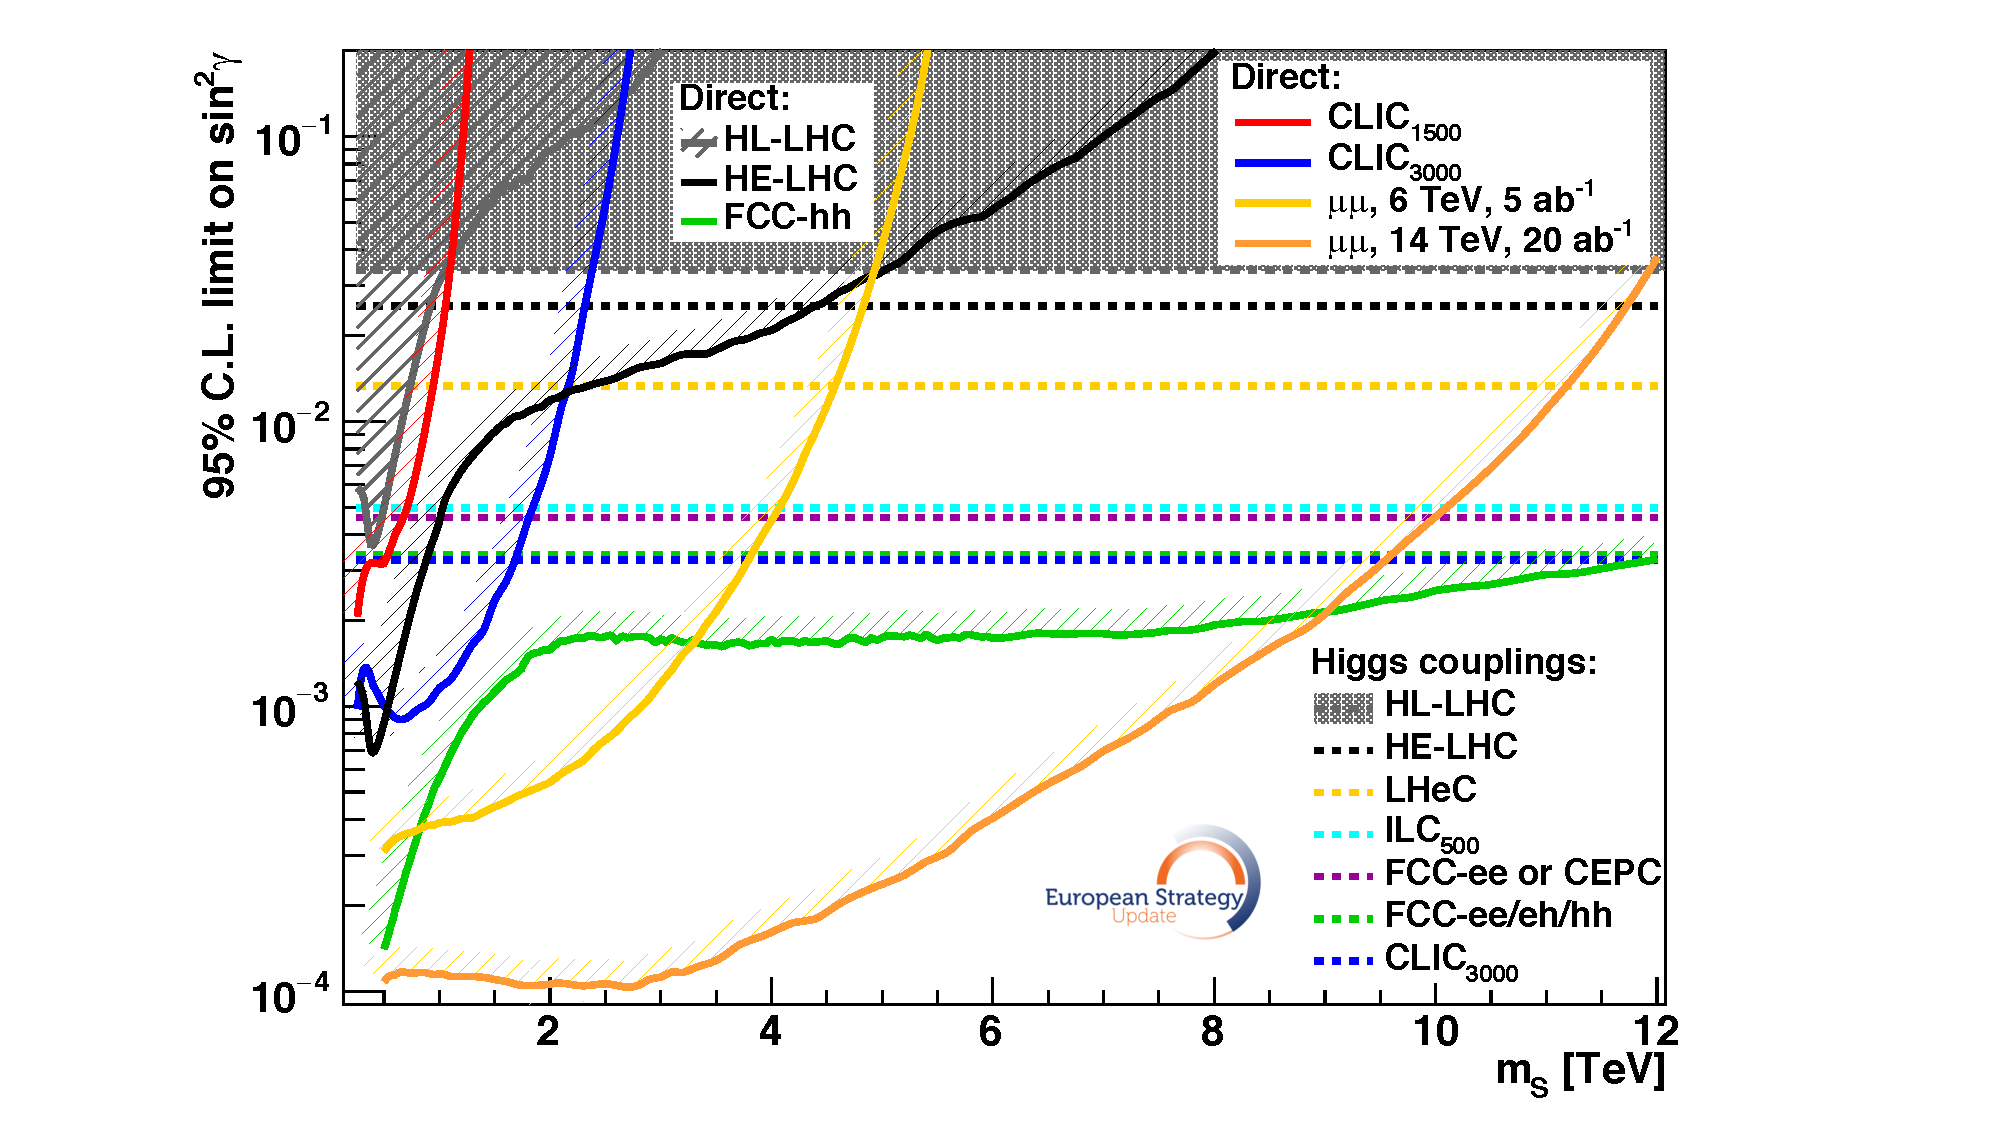
\includegraphics[width=0.49\textwidth]{\main/BSM/ExtendedScalars/singlet_all_options-2.pdf}
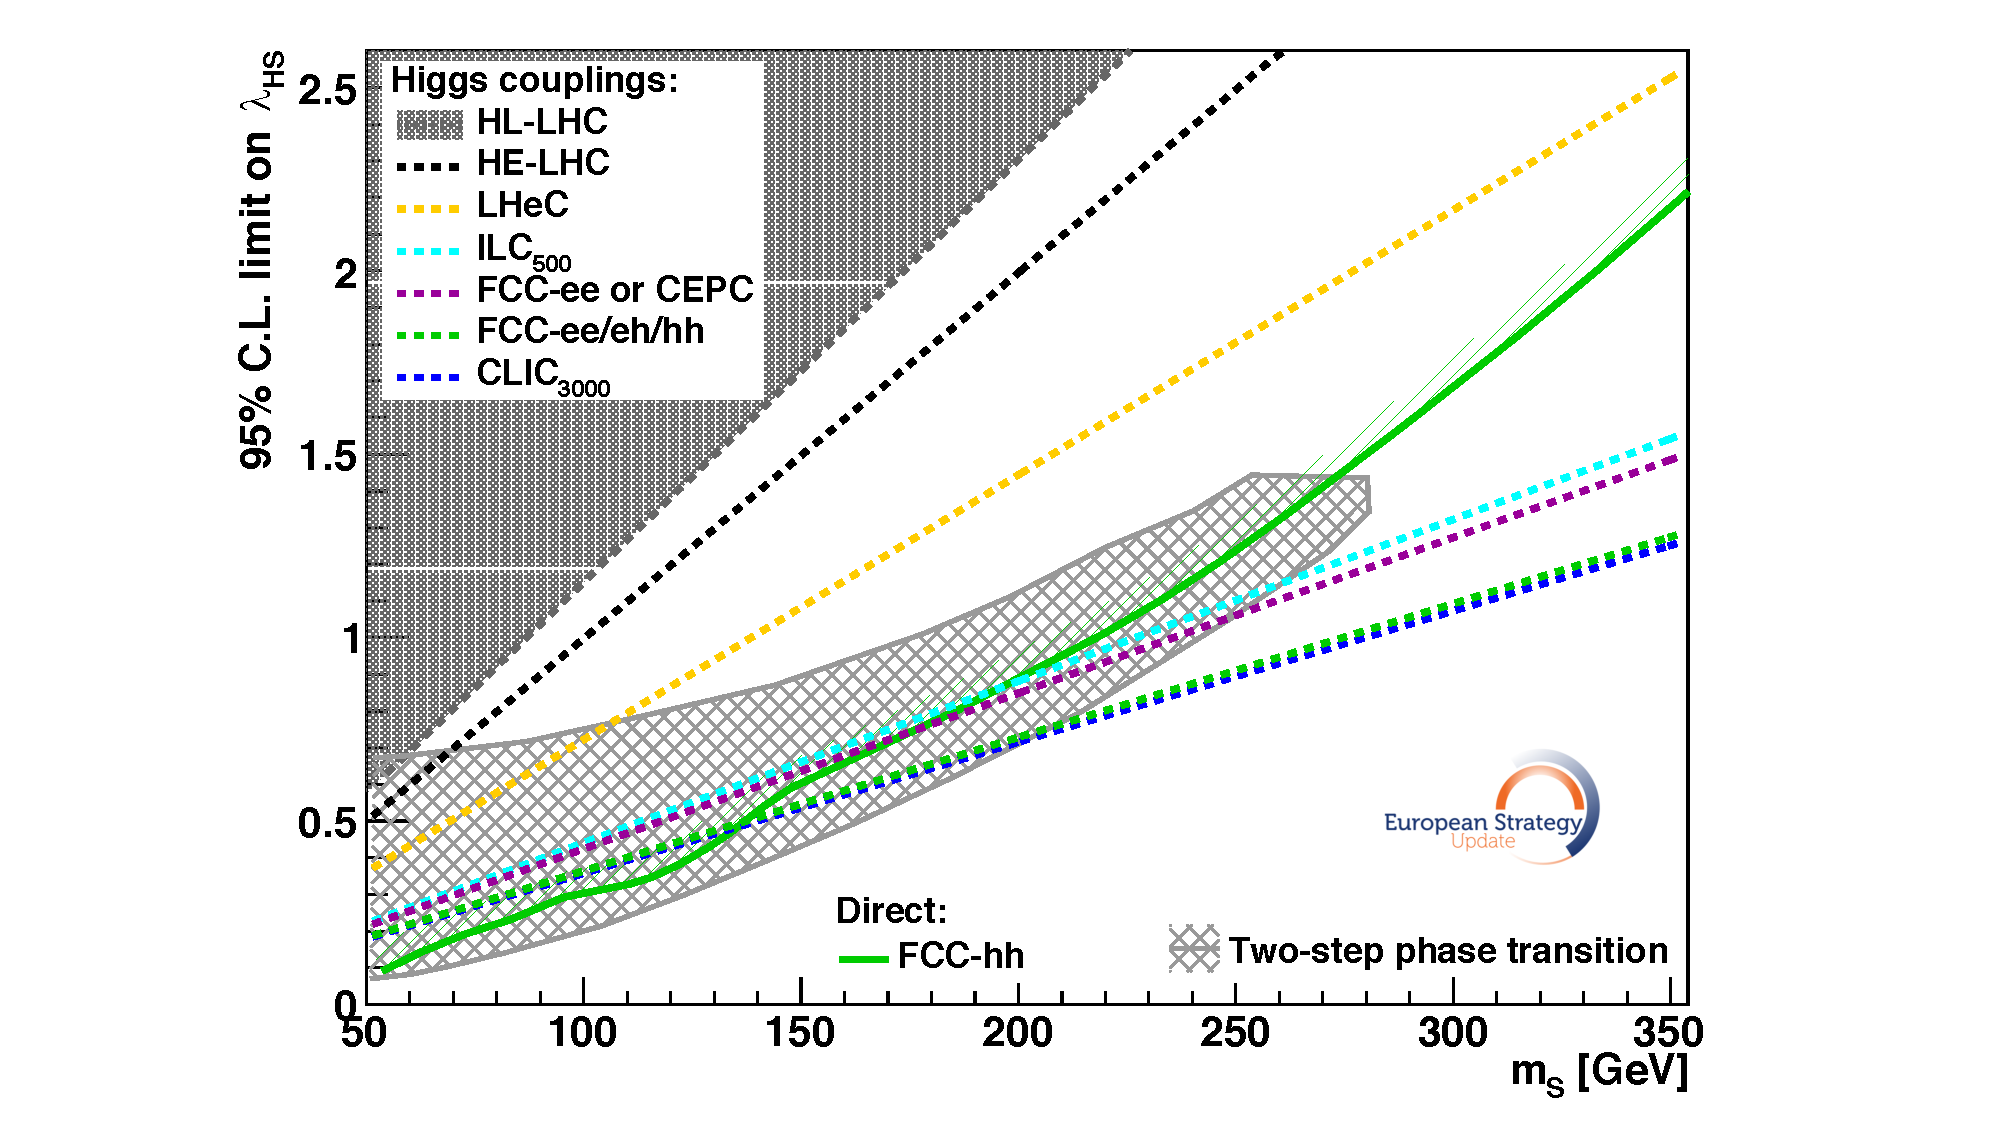
\includegraphics[width=0.49\textwidth]{\main/BSM/ExtendedScalars/singlet_no_mixing.pdf}
\caption{Direct and indirect sensitivity at 95\% CL to a heavy scalar singlet mixing with the SM Higgs boson (left) and in the no-mixing limit (right). The hatched region shows the parameters compatible with a strong first-order EW phase transition.}
\label{fig:singlets}
\end{figure}

In the no-mixing case, in which $S$ does not acquire a vacuum expectation value and the $Z_{2}$ symmetry remains unbroken, the new scalar is stable and escapes undetected. Figure~\ref{fig:singlets} (right) shows the indirect sensitivity on the coupling $\lambda_{HS}$ from the overall scaling of the Higgs couplings. The figure also shows the reach using the VBF process $pp \rightarrow SSjj$ at \FCChh~\cite{Curtin:2014jma}, which provides the best direct sensitivity in hadron collisions. It is interesting to note that a large fraction of the region compatible with a first-order phase transition could be probed by the full CLIC or FCC programmes. For illustration purposes, Fig.~\ref{fig:singlets} shows an example of the region compatible with a two-step phase transition, where the singlet supports the Higgs in delivering a strong first-order phase transition~\cite{Chala:2018opy}. 
%which could in turn help our understanding of the matter-antimatter asymmetry of the Universe~\cite{Chala:2018opy} 
Strongly first-order phase transitions are particularly interesting as they could also lead to sizeable gravitational wave signals at future experiments like LISA, linking discoveries at Earth-based colliders with space interferometry (see Chapter~\ref{chap:cosm}).

\begin{figure}[ht]
\centering
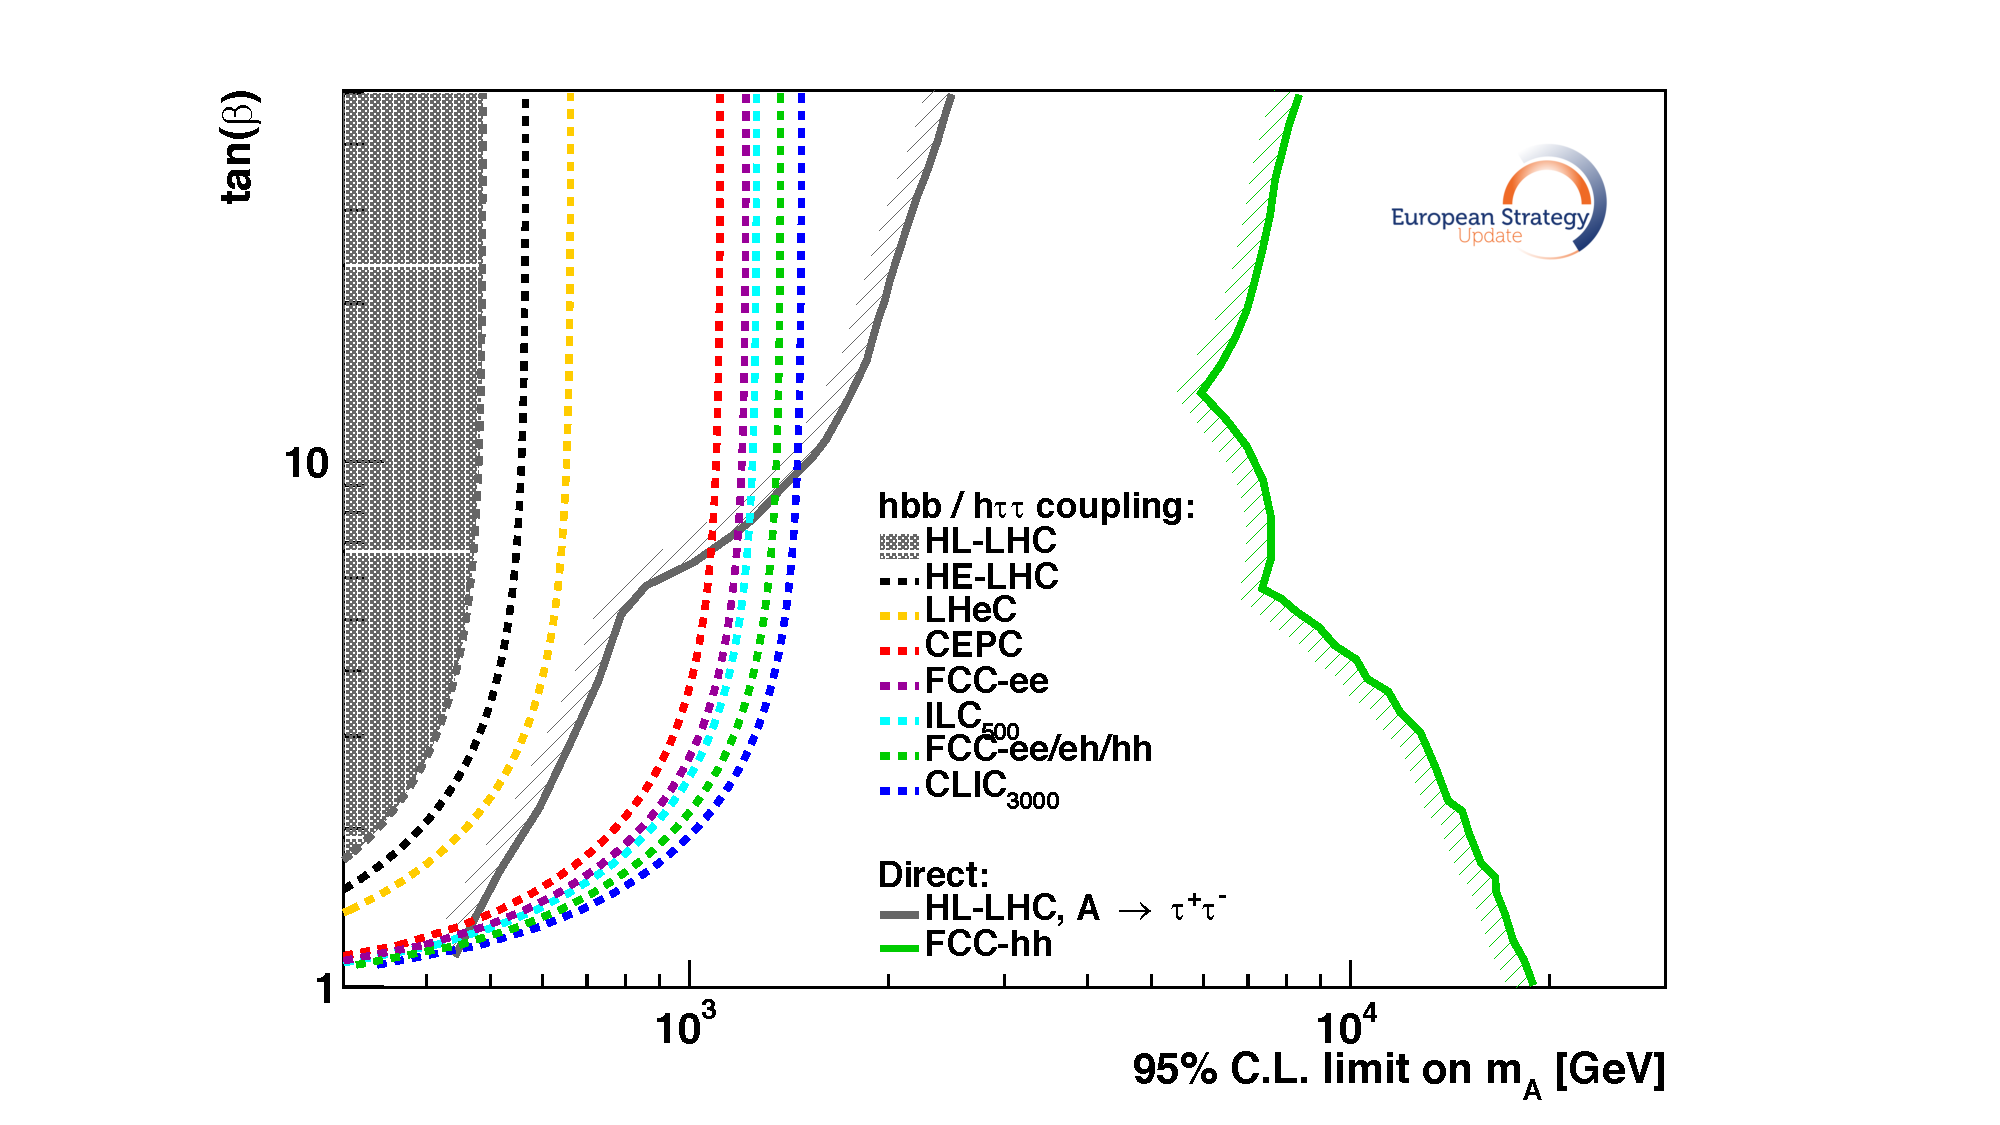
\includegraphics[width=0.7\textwidth]{\main/BSM/ExtendedScalars/2hdm_all.pdf}
%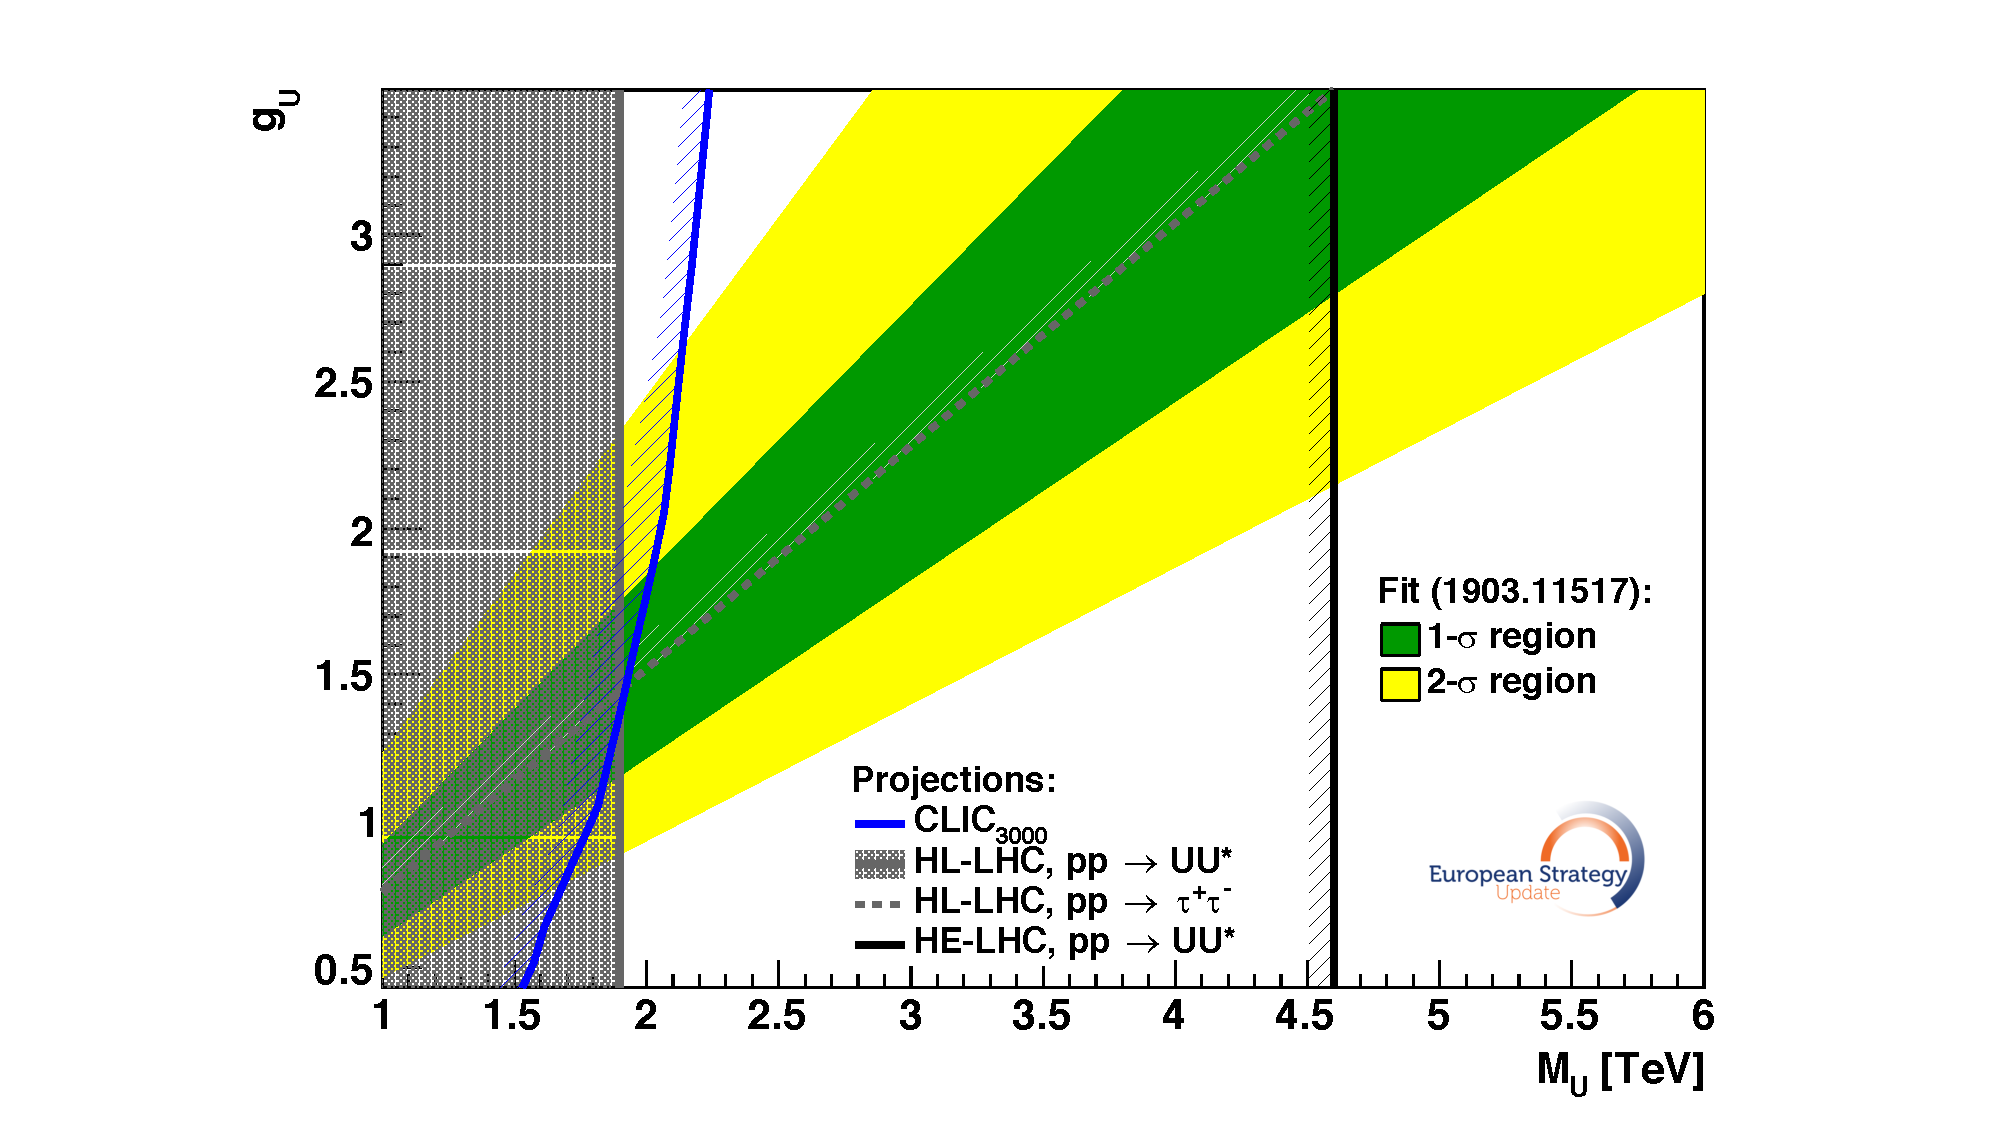
\includegraphics[width=0.49\textwidth]{\main/BSM/ExtendedScalars/u1_leptoquark_all.pdf}
\caption{Direct and indirect sensitivity at 95\% CL to heavy neutral scalars in minimal SUSY. 
%Reach for the vector leptoquark $U_{1}$ in the mass versus coupling plane (right).
}
\label{fig:2hdm}
\end{figure}

Another common extension of the SM Higgs sector is the addition of a second SU(2) doublet, which naturally appears in supersymmetric extensions of the Higgs sector or in  models with a non-minimal pattern of symmetry breaking. In this case, the scalar sector contains two CP-even scalars $h$ and $H$, one CP-odd scalar $A$ and a charged scalar $H^{\pm}$. The direct mass reach of lepton colliders for these scalars is generally close to $\sqrt{s}/2$ independent of $\tan{\beta}$, mainly using $e^{+}e^{-} \rightarrow H^{+}H^{-}$ and $e^{+}e^{-} \rightarrow AH$. The cross sections for these processes are almost independent of the heavy Higgs boson masses for a given $\sqrt{s}$. As expected, the highest mass reach is obtained at hadron colliders. 

A well-studied example of a Type-II Two-Higgs Doublet Model is the minimal SUSY extension of the SM. The \HLLHC is sensitive to heavy neutral scalars up to 2.5~TeV for $\tan{\beta} > 50$ using $A/H \rightarrow \tau^{+}\tau^{-}$ decays~\cite{Curtin:2014jma} while the region of low $\tan{\beta}$ can be probed with decays to top-quark pairs. At \FCChh, the expected 95\% CL exclusion limits for the $H/A$ states are generally better than 5\,TeV and extend up to 20\,TeV for low $\tan{\beta}$~\cite{Craig:2016ygr}. These projections are compared in Fig.~\ref{fig:2hdm} to the indirect sensitivity on $m_{A}$ from Higgs couplings to third-generation fermions~\cite{Gunion:2002zf, Gorbahn:2015gxa}. While for a given lepton collider $g_{hbb}$ is the most precise option, hadron colliders provide better accuracy on $g_{h\tau\tau}$~\cite{deBlas:2019rxi}. Hence the more precise of the two couplings was chosen to calculate the limit for each collider scenario. A global analysis of all Higgs observables would improve the indirect sensitivity further. The corresponding \FCChh sensitivity for the charged $H^{\pm}$ particles are in the range from 10 to 15\,TeV~\cite{Hajer:2015gka}.

Doubly-charged Higgs bosons exist in Type-II seesaw models, where a new scalar triplet could couple to the SM leptons to produce the light neutrino masses. For low values of the vacuum expectation value of the triplet ($v_{\Delta}$) the doubly-charged Higgs bosons would decay leptonically. Polarisation measurements in decays to $\tau$ leptons can help discriminate between different heavy scalar mediated neutrino mass models. An interesting case is the region where $v_{\Delta}$ is relatively large and the doubly-charged Higgs would decay into two same-sign W bosons. Lepton colliders could reach masses almost up to the kinematic limit of $\sqrt{s}/2$ using $e^{+}e^{-} \rightarrow H^{++}H^{--}$ events~\cite{Agrawal:2018pci}. The \FCChh would be sensitive to $H^{++}H^{--} \rightarrow W^{+}W^{+}W^{-}W^{-}$ for doubly charged Higgs masses up to 1.7\,TeV and $v_{\Delta} > 10^{-4}$\,GeV~\cite{Du:2018eaw}.

\subsection{Neutral naturalness}
Neutral naturalness (NN) describes the class of theories in which the top-quark partner, needed to regulate the leading SM quantum corrections to the Higgs mass, is colour neutral. This makes NN theories particularly elusive to LHC direct searches. The prototype model of NN is the Twin Higgs~\cite{Chacko:2005pe}, which introduces a mirror copy of the SM with twin particles and a twin gauge group. The SM and its mirror copy are related by a discrete symmetry that ensures equal coupling constants between the two sectors. As a result of the doubling of states, the scalar potential has an enlarged accidental global symmetry which, after spontaneous symmetry breaking, leads to a Goldstone boson with the right quantum numbers to be identified with the SM Higgs. Since the accidental symmetry is not exact in the full theory, the Higgs acquires a mass at the loop level, but its value is smaller than the cutoff thanks to an approximate cancellation between the contributions from SM and twin-sector particles. In the Twin Higgs, the top-quark partner is a new EW-neutral fermion, but NN variations can turn the top-partner into an EW-charged scalar (Folded SUSY~\cite{Burdman:2006tz}), an EW-charged fermion (Quirky Little Higgs~\cite{Cai:2008au}), or an EW-neutral scalar (Hyperbolic Higgs~\cite{Cohen:2018mgv,Cheng:2018gvu}). 

The NN top-partners are expected to have masses around $m_T \approx \sqrt{1/\epsilon}$~500~GeV, where $\epsilon$ is the degree of fine tuning. If they carry EW charge, the NN top-partners can be produced at colliders via DY-like processes. However, because of their unavoidable couplings with the Higgs, a more robust way of detecting their presence is through Higgs precision measurements. Since the parametric scaling of Higgs coupling modifications in NN is identical to the case of Composite Higgs, the reach of future colliders on the degree of tuning $\epsilon$ of NN theories can be read from Fig.~\ref{fig:Composite_Higgs_Summary} (blue bars, right axis).

NN theories can address the naturalness problem without coloured particles at the weak scale, but require a completion at a nearby mass scale $m_{\rm NN}$, where new coloured states are expected. This mass scale is model dependent, but it is generally in the range $m_{\rm NN}\approx \sqrt{0.1/\epsilon}$~3--5~TeV. This shows that, for moderate tuning, the NN coloured particles are beyond the reach of the LHC but are perfect targets for high-energy future colliders. 
The states in the twin sector that communicate with the SM only through the Higgs can lead to unusual signatures. An interesting case are the twin glueballs, which are expected to be light and typically long-lived. They can be produced in Higgs decays and then decay back into SM states, leading to distinguishing vertex displacements that can be hunted for in main detectors or, depending on the lifetime, with dedicated detectors far from the interaction point such as MATHUSLA200. Searches for invisible Higgs decays also contribute to the exploration of the parameter space.

\subsection{High-energy flavour dynamics}
Heavy new physics can induce, through the exchange of virtual particles, processes that are extremely rare in the SM, such as FCNC effects in the top-quark sector (see also Chapter~\ref{chap:flav}). Experimental projections on searches for rare FCNC top-quark decays are available for many of the proposed projects. Complementary sets of measurements using various top-quark production processes and decays are accessible in $e^+e^-$, $ep$ and $pp$ collisions. The projections are summarised in Table~\ref{tab:top_fcnc_decays}. While not all possibilities have been explored yet, generally improvements of 1--2 orders of magnitude are possible compared to \HLLHC.

\begin{table}
\caption{Limits on FCNC top-quark decays at 95\% CL for various future colliders~\cite{Cerri:2018ypt, Bambade:2019fyw, Abramowicz:2018rjq, Khanpour:2014xla, Abada:2019lih}. Results are also given for flavour-inclusive final states with $q = u, c$. Empty entries correspond to cases in which studies are not available at the time of writing.}
\centering
\begin{tabular}{ c | c | c | c | c | c | c | c | c }
$BR \times 10^{5}$ & \HLLHC & \HELHC & \ILCFiveHundred & \CLICThreeHundredEighty & LHeC & \FCCee & \FCChh & \FCCeh \\
\hline
$t \rightarrow Hc$ & & & $\approx 3$ & 15 & & & 1.6 & \\
$t \rightarrow Hu$ & & & & & 150 & & & 22 \\
$t \rightarrow Hq$ & 10 & & & & & & 2.8 & \\
\hline
$t \rightarrow Zq$ & 2.4 - 5.8 & & & & 4 & 2.4 & $\approx 0.1$ & 0.6 \\
\hline
$t \rightarrow \gamma c$ & 7.4 & & $\approx 1$ & 2.6 & & & 0.024 & \\
$t \rightarrow \gamma u$ & 0.86 & & & & & & 0.018 & \\
$t \rightarrow \gamma q$ & & & & & 1 & 1.7 & & 0.085 \\
\hline
$t \rightarrow gc$ & 3.2 & 0.19 & & & & & & \\
$t \rightarrow gu$ & 0.38 & 0.056 & & & & & & \\
\end{tabular}
\label{tab:top_fcnc_decays}
\end{table}

At lepton colliders, the process $e^{+}e^{-} \rightarrow tj$ is much more powerful compared to tests on top-quark decays, which are limited by statistics. In particular, operation at the highest possible energies improves the sensitivity to four-fermion operators. The full CLIC programme would be sensitive to operator scales in the region of 50--100~TeV~\cite{deBlas:2018mhx}.

\begin{figure}[ht]
\centering
%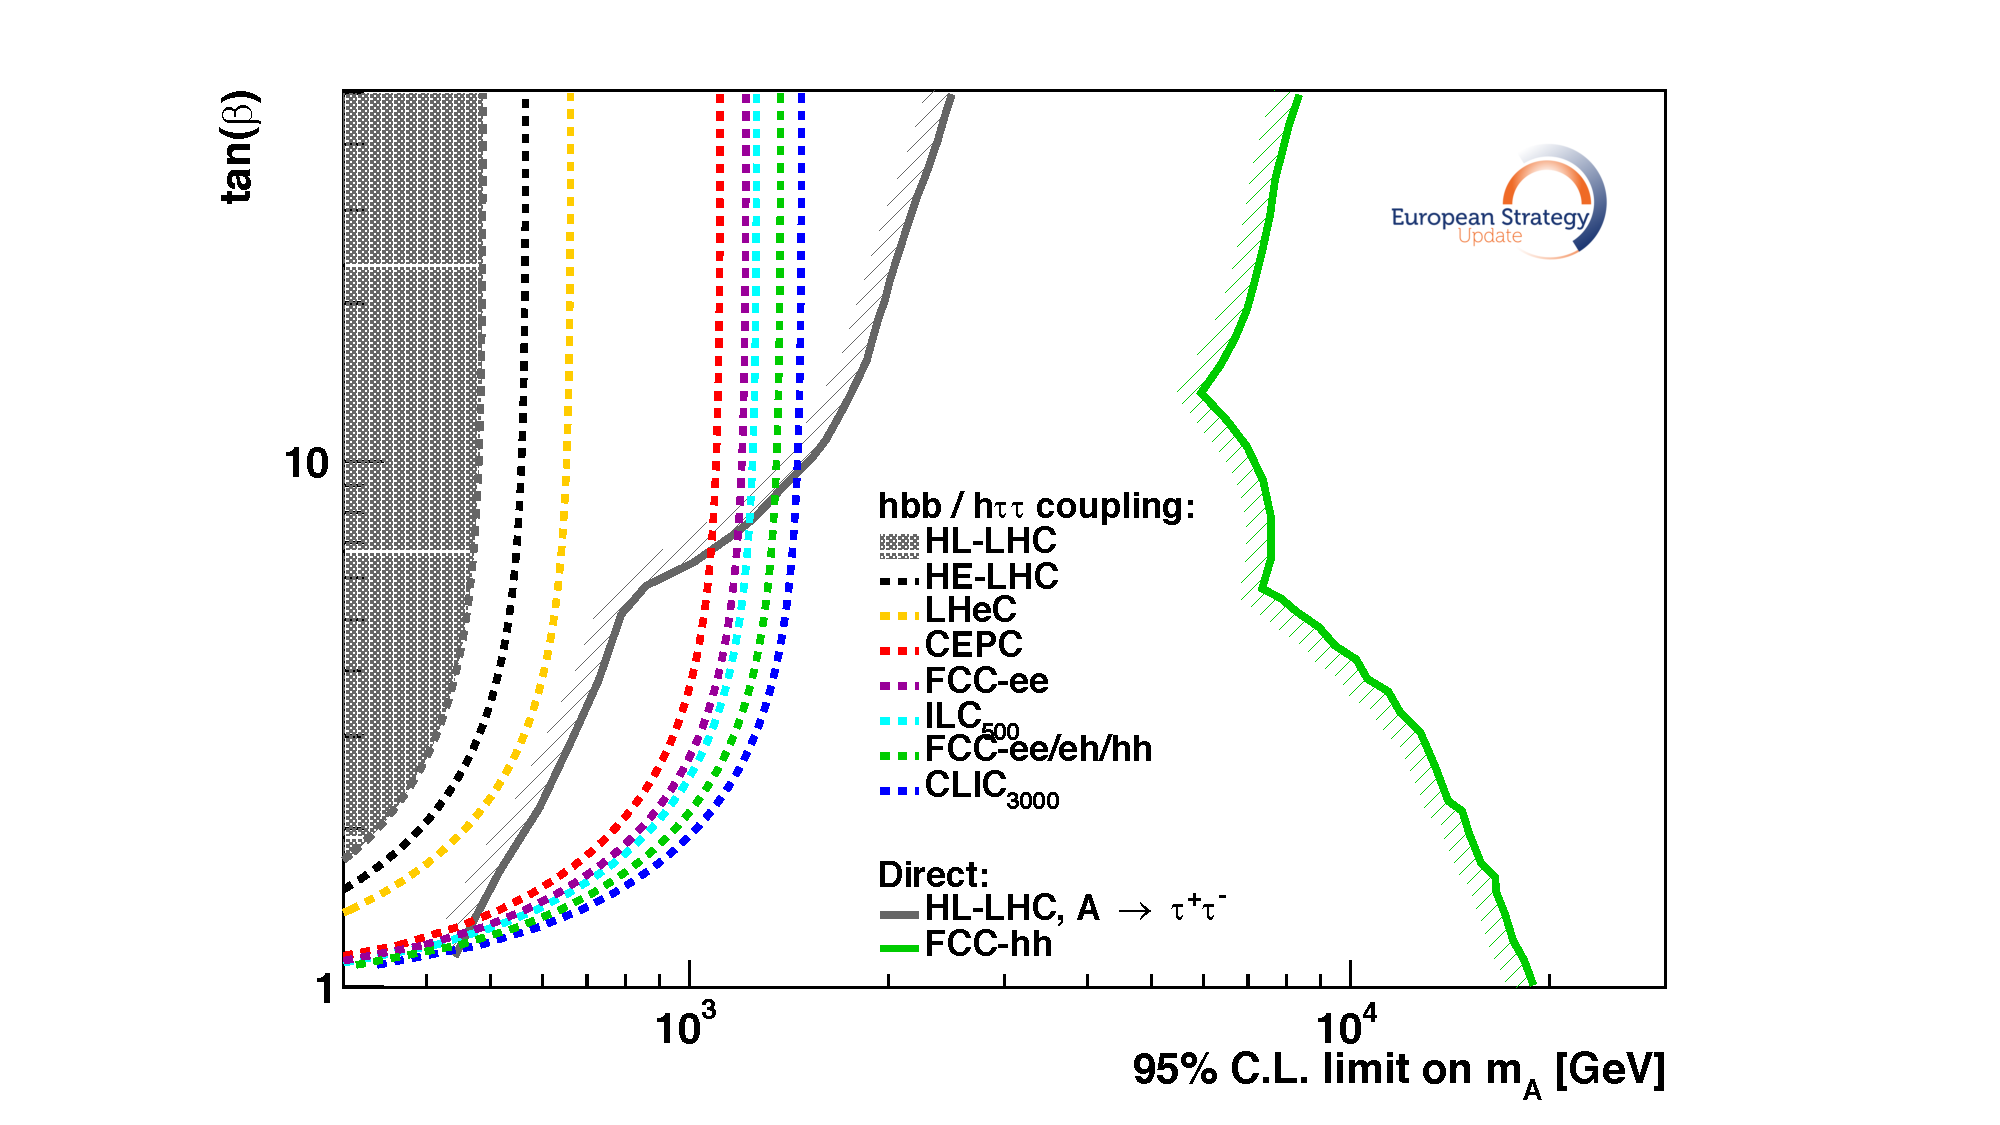
\includegraphics[width=0.49\textwidth]{\main/BSM/ExtendedScalars/2hdm_all.pdf}
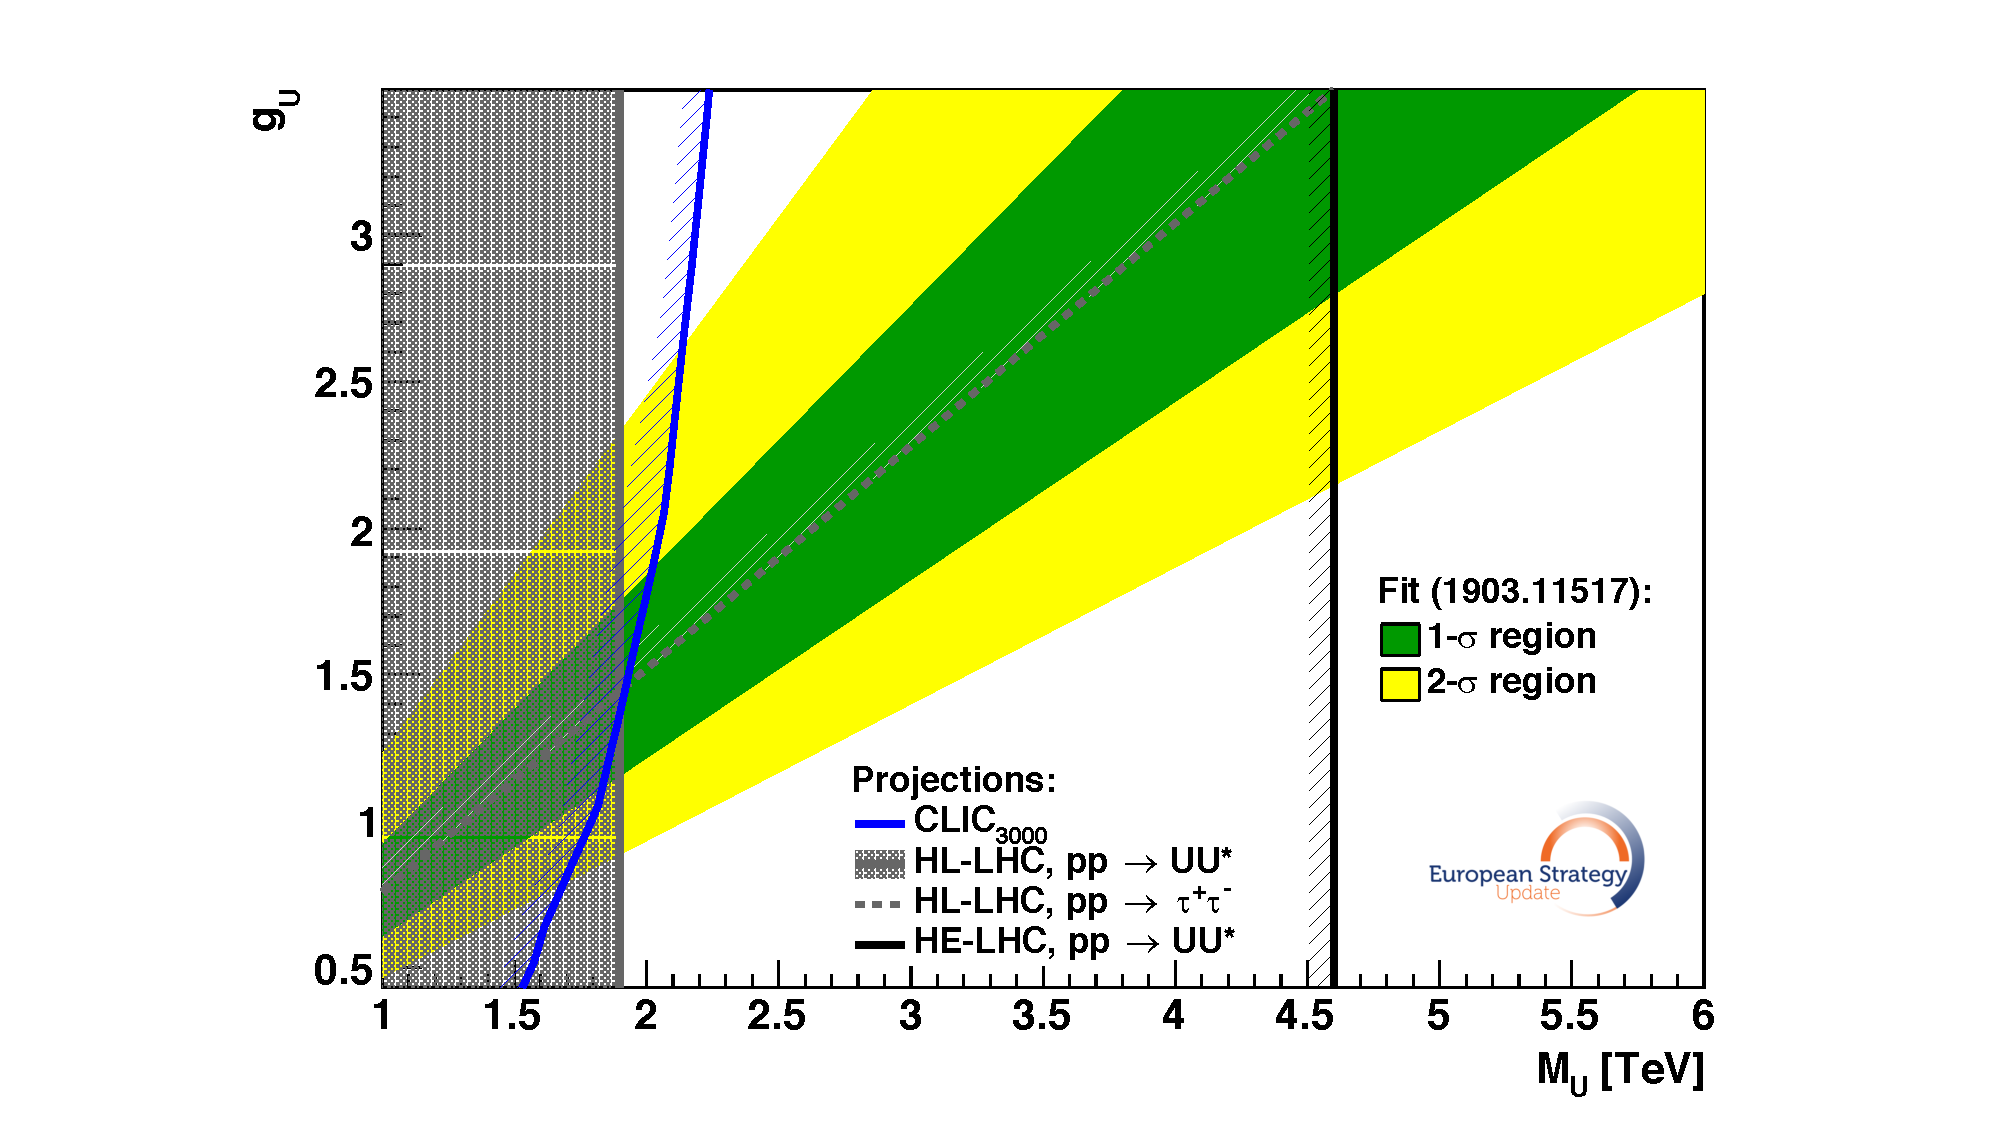
\includegraphics[width=0.7\textwidth]{\main/BSM/ExtendedScalars/u1_leptoquark_all.pdf}
\caption{
%Direct and indirect sensitivity at 95\% CL to heavy neutral scalars in minimal SUSY (left). 
Direct and indirect sensitivity at 95\% CL for the vector leptoquark $U_{1}$ in the mass versus coupling plane.}
\label{fig:leptoquarks}
\end{figure}

Renewed interest in leptoquarks was triggered by recent results in rare $B$ decays, which show discrepancies with respect to the SM predictions. For example, the $b \rightarrow c\tau\nu$ results are presently compatible with a rather light leptoquark coupled predominantly to the third generation. The mass reach from QCD pair-production of the scalar leptoquark $S_{3}$ or vector leptoquark $U_{1}$ at \HLLHC is 1.5--2.0~TeV~\cite{CidVidal:2018eel}, independently of the coupling to the lepton-quark current. Complementary information would be provided in the large-coupling region by the process $pp \rightarrow \tau^{+}\tau^{-}$. A modest improvement in sensitivity for the $S_{3}$ would be provided by CLIC~\cite{deBlas:2018mhx}. The highest mass reach is available at hadron colliders. For example, \HELHC would improve the direct mass reach by more than a factor two compared to \HLLHC. Projections for the different colliders in the $U_{1}$ case are shown and compared to a recent global flavour fit~\cite{Cornella:2019hct} in Fig.~\ref{fig:leptoquarks}.

\end{document}

